\documentclass{standalone}
\usepackage{tikz}

\begin{document}
	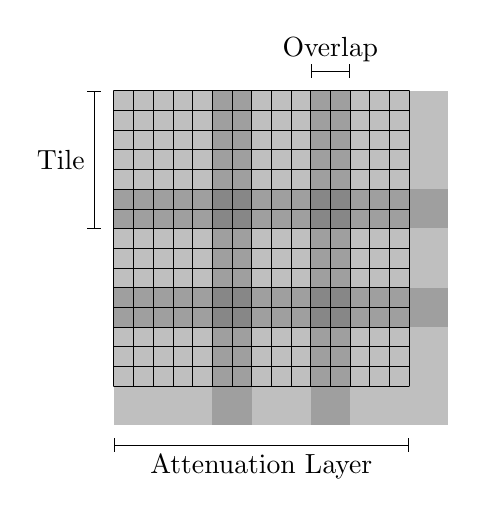
\begin{tikzpicture}[scale = 0.25, very thin]
	
		% Tiles
		\foreach \x in {0,...,2} {
			\foreach \y in {0,...,2}{
				\fill[gray, opacity = 0.5] (\x * 5, -\y * 5) rectangle ++(7, -7);
			}
		}
		
		% Grid
		\draw[step = 1 cm, cap = round] (0, 0) grid (15, -15);
		
		% Markers
		\draw[|-|] (0, -18) -- node[below]	{Attenuation Layer} ++(15, 0);
%		\draw[|-|] (18, 0) -- node[right]	{$R_y$} ++(0, -15);
%		\draw[|-|] (0, 1) 	-- node[above]	{Tile} ++(7, 0);
		\draw[|-|] (-1, 0) 	-- node[left]	{Tile} ++(0, -7);
		\draw[|-|] (10, 1) 	-- node[above]	{Overlap} ++(2, 0);
%		\draw[|-|] (-1, -10) -- node[left]	{$o_y$} ++(0, -2);
	
	\end{tikzpicture}
\end{document}
